\section{Creazione della scena}
\label{sec:chapter_caso_uso_creazione_scena}

L’utente che vuole realizzare una scena 3D usufruendo del servizio Editor deve accedere al servizio mediante apposita URL.
Una volta acceduto al servizio, l’utente può iniziare il processo di realizzazione; tale processo si decompone in una successione di operazioni, che possono essere svolte in qualsiasi ordine.
\\
In questo paragrafo verranno quindi presentate le operazioni effettuabili durante una tipica esperienza d’uso dell’editor da parte dell’utente. 
L’esperienza che verrà mostrata sarà relativa alla release attuale del servizio.
Il processo di realizzazione di una scena 3D passa inevitabilmente per una fase di inserimento dei modelli che la comporranno. 
\\
Per inserire un modello l’utente ha la possibilità di importare un file JSON o OBJ di un modello già pronto, mediante la funzionalità \emph{LOAD} nel menu \emph{FILE}. 
L’utente ha inoltre la possibilità di usufruire di un catalogo di modelli gia pronti; per accedere al catalogo, l’utente seleziona la voce \emph{OPEN CATALOG} nel menù \emph{FILE}. Una volta aperto il catalogo l’utente può cliccare sull’immagine del modello desiderato per visualizzare un'anteprima di come apparirà il modello 3D, con la relativa texture, all'interno della scena.
A questo punto l'utente può aggiungere l'oggetto alla scena, selezionando la voce \emph{ADD TO SCENE}. 
\\
\begin{figure}[htb]
 \centering
 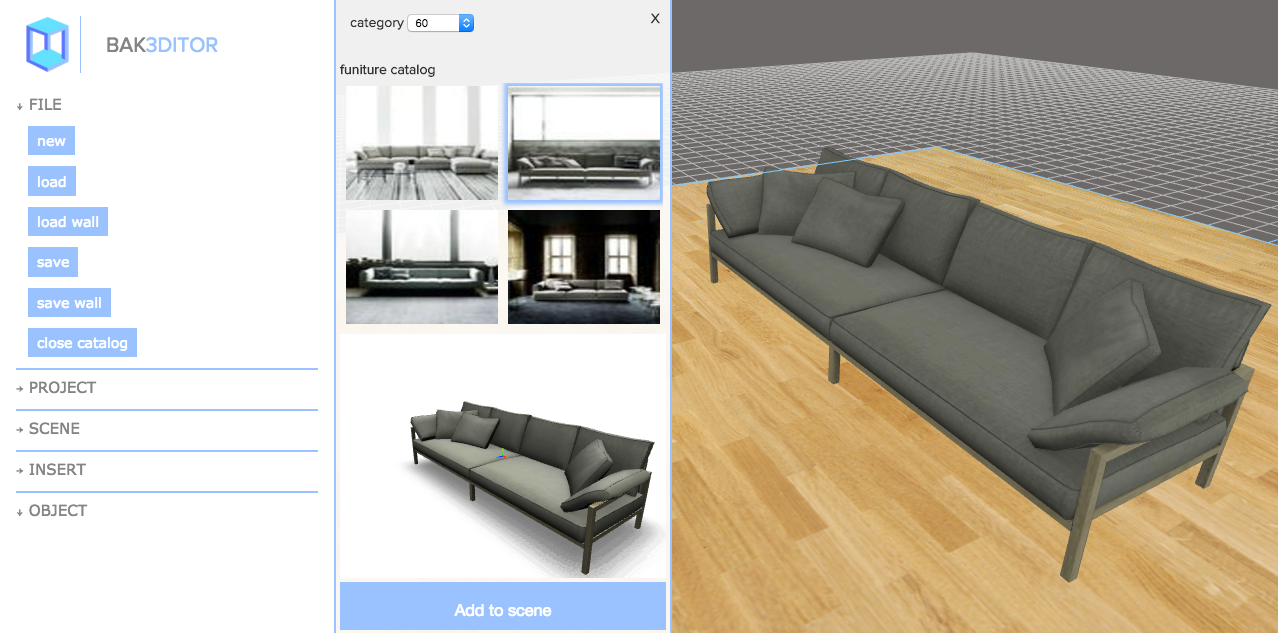
\includegraphics[width=1\linewidth]{images/chapter_caso_uso/caso_uso_catalogo.png}\hfill
 \caption[Catalogo prodotti]{Dettaglio dell'Editor riguardante il catalogo prodotti, con la possibilità di visionare un'anteprima dell'oggetto prima di aggiungerlo alla scena.}
 \label{fig:caso_uso_catalogo}
\end{figure}
Oltre all’import di modelli già pronti, l’Editor offre la possibilità di crearli. Per creare un modello, nel menù \emph{INSERT/GEOMETRY} l’utente può selezionare la voce inerente alla geometria che si vuole aggiungere per il modello. In corrispondenza di ogni voce, l’utente può regolare le dimensioni della geometria, in modo da importarla già delle dimensioni desiderate.
Oltre alle geometrie tradizionali (sfera, cubo, piano) l’editor permette di importare degli oggetti “muro”.
\\
Selezionando la voce \emph{WALL} dal menu \emph{GEOMETRY} l’utente importa nella scena un oggetto nel quale è possibile regolare la posizione e la dimensione di una cavità, nella quale inserire eventuali porte o finestre. Una volta regolata la cavità l’utente seleziona la voce \emph{CREATE}, e l’editor genera l’oggetto muro definitivo.
\\
\begin{figure}[htb]
 \centering
 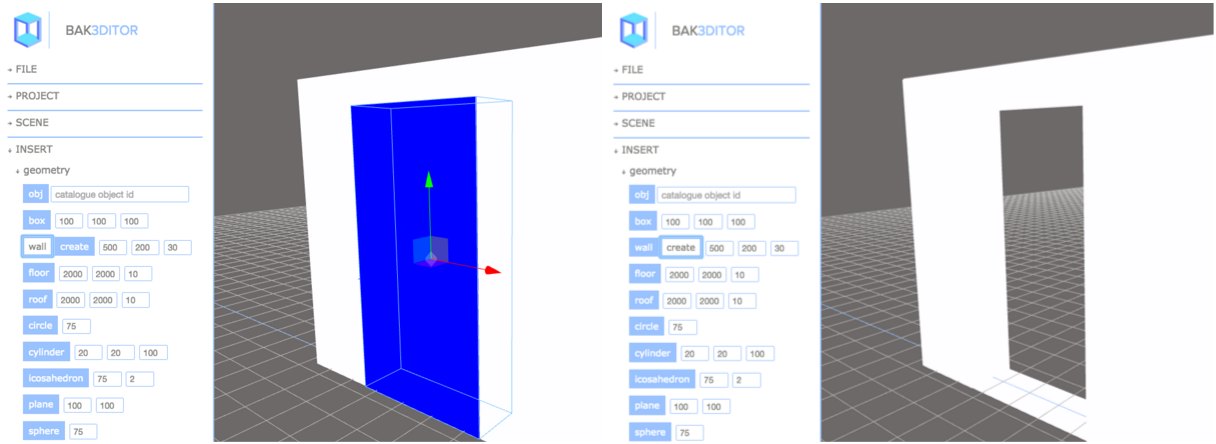
\includegraphics[width=1\linewidth]{images/chapter_caso_uso/caso_uso_muri.png}\hfill
 \caption[Costruzione muri]{Funzionalità WALL dell'editor per la realizzazione di muri all'interno della scena}
 \label{fig:caso_uso_muri}
\end{figure}
Qualsiasi modello presente all’interno della scena può essere ruotato, scalato, o traslato dal’utente. Qualsiasi trasformazione è possibile su un oggetto solo se l’oggetto è selezionato.
\\
Le opzioni di trasformazione possono essere scelte dal menu \emph{PROJECT/TRANSFORM}, oppure richiamate direttamente mediante shortcut da tastiera: per traslare l’oggetto l’utente può premere il tasto \emph{G}, per ruotarlo \emph{R}, e per scalarlo \emph{S}. In qualsiasi momento durante la trasformazione di un oggetto l’utente può consultare i pannelli \emph{POSITION}, \emph{ROTATION} e \emph{SCALE} dal menu \emph{OBJECT/MESH}. Questi pannelli sono aggiornati in tempo reale sui valori numerici di rotazione, scalatura, e traslazione lungo i tre assi \emph{X,Y,Z}. 
\\
L’utente può inoltre interagire direttamente con i pannelli, inserendo i valori numerici di trasformazione senza quindi doverla effettuare a mano.
\\
In qualsiasi momento un oggetto può essere duplicato o rimosso dalla scena cliccando la voce \emph{CLONE} o emph{REMOVE} nel menu \emph{OBJECT/MESH}, o premendo da tastiera rispettivamente il tasto \emph{D} per la duplicazione, o \emph{X} per la rimozione.
\\
Una volta che l’utente ha aggiunto un modello all’interno della scena, può regolarne il materiale dal menu \emph{OBJECT/MATERIAL}. Il menu offre tutte le opzioni di configurazione tipiche di un materiale, come la scelta del tipo di materiale, del colore, del valore di brillantezza o di trasparenza.
\\
La regolazione dei materiali passa anche per la texturizzazione. 
Una volta selezionato l’oggetto, sempre dal menu \emph{OBJECT/MATERIAL} l’utente può mappare una texture, una ligtmap o altri tipi di immagini. Ad esempio una diffuse texture viene applicata cliccando \emph{LOAD} in corrispondenza della voce \emph{MAP}, e selezionando dal file system l’immagine che si vuole utilizzare come diffuse texture. 
\newpage
\begin{figure}[htb]
 \centering
 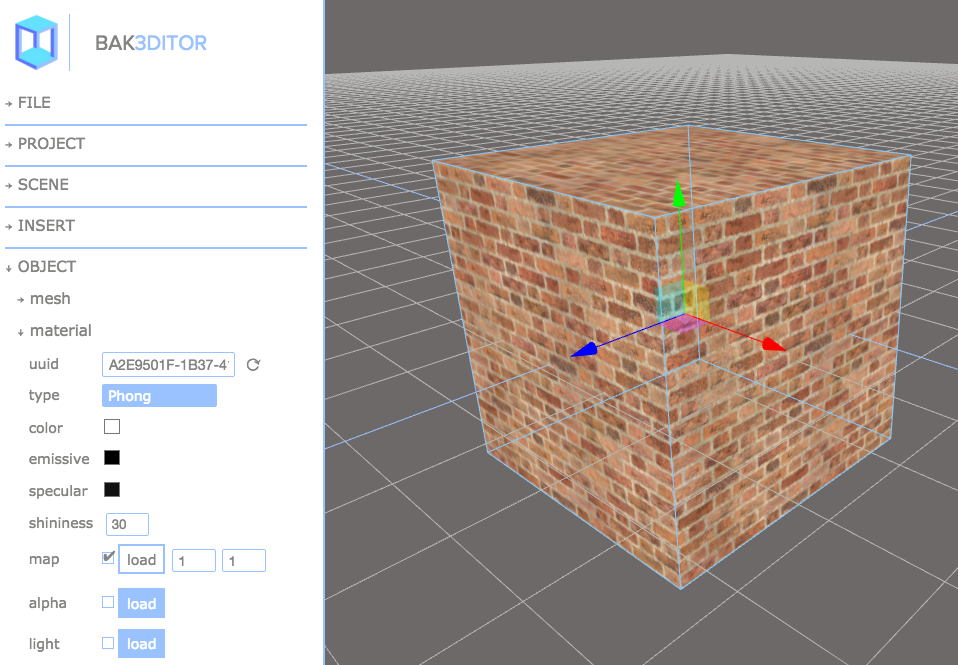
\includegraphics[width=0.7\linewidth]{images/chapter_caso_uso/caso_uso_texture.png}\hfill
 \caption[Texturizzazione]{Texturizzazione di un cubo mediante apposita funzionalità offerta dall'editor.}
 \label{fig:caso_uso_texture}
\end{figure}
Per realizzare effetti di riflessione e rifrazione sulla superficie dell’oggetto, il menu \emph{OBJECT/MATERIAL} offre la possibilità di importare delle env map sempre da file system. 
\\
Tuttavia l’utente ha la possibilità di generare un’env map direttamente dall’editor, cliccando in corrispondenza della voce \emph{ENV} sull’opzione \emph{REFR} per generare una env map di rifrazione, o sull’opzione \emph{REFL} per generare una env map d riflessione; l’env map viene automaticamente generata e applicata sulla superficie oggetto selezionato.
\\
\begin{figure}[htb]
 \centering
 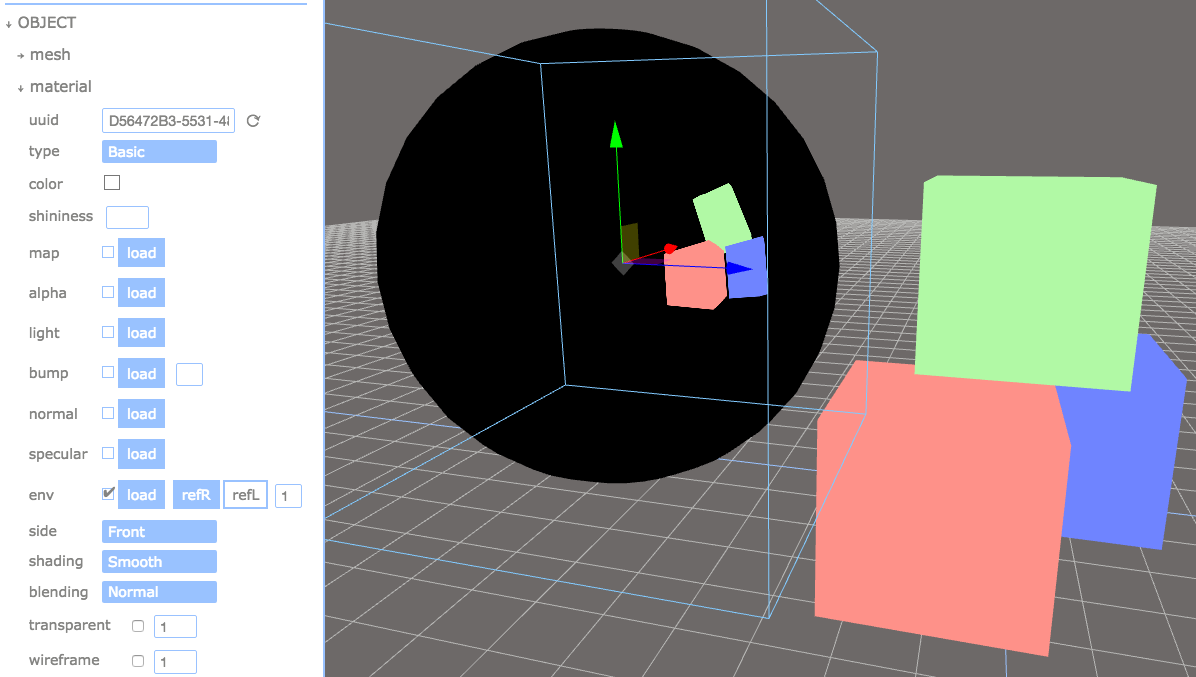
\includegraphics[width=0.8\linewidth]{images/chapter_caso_uso/caso_uso_envmap.png}\hfill
 \caption[Effetti riflessione/rifrazione]{Realizzazione di un'env map di riflessione applicata sulla sfera.}
 \label{fig:caso_uso_envmap}
\end{figure}
\\
Nell’ipotesi in cui l’utente desideri effettuare il bake della scena, l’Editor offre una serie di parametri aventi come obiettivo quello di regolare la partecipazione dell’oggetto selezionato al processo di bake. Tali parametri sono \emph{AVOID\_BAKE} e \emph{PROJECT\_SHADOW}, e si trovano nel menu \emph{OBJECT/MESH}.
\\
Durante la generazione della scena l’utente può consultare la gerarchia degli oggetti che ha inserito. Questa gerarchia è mostrata nel menu \emph{SCENE} dell’Editor. 
\\
Selezionare il nome dell’oggetto dal pannello della gerarchia equivale a selezionare l’oggetto vero e proprio. 
Inoltre in qualsiasi momento l’utente può abilitare una modalità \emph{HELPER} dell’Editor; questa modalità è utile per aiutare l’utente nell’individuare e posizionare gli oggetti nella scena, specialmente se sono molti.
Inoltre, l’editor offre la possibilità di consultare una mappa 2D della scena vista dall’alto, per poterla osservare da un punto di vista differente.
\\
Quando l’utente ha terminato la realizzazione della scena può decidere di salvare il risultato, che viene esportato nel formato di interscambio dei dati visto nel paragrafo \ref{sec:chapter_architettura_sistema_formato_scambio}.
\\
La scena esportata può essere reimportata in qualsiasi momento nell’editor, anche in sessioni differenti. Inoltre il file JSON contenente la scena può essere passato a terzi, che a loro volta possono decidere di importarlo nel loro Editor.
